\section{Statistics}


%%%%%%%%%%%%%%%%%%%%%%%%%%%
%
% Probability Distributions
%
%%%%%%%%%%%%%%%%%%%%%%%%%%%

\formdesc{Expected Value}

\begin{equation}
	E(X) = \mu = \sum_{i=1}^k x_i ~ P(X = x_i)
\end{equation}

for a discrete random variable with $k$ possible values.
\hformbar




\formdesc{General Variance Formula}

\begin{equation}
	Var(X) = \sigma^2 = \sum_{j=1}^k (x_j - \mu)^2 ~ P(X = x_j),
\end{equation}

or, the sum of the squared deviations $(x_j - \mu)^2$ weighted by the corresponding probabilities $P(X=x_1),  \ldots, P(X=x_k)$.
\hformbar



\formdesc{General Standard Deviation}

\begin{equation}
	\sigma = \sqrt{\sigma^2} = \sqrt{Var(X)}
\end{equation}
\hformbar



\formdesc{Linear Combinations of Variables}

\begin{equation}
	Z = aX + bY
\end{equation}

is a linear combination of the independent, random variables $X$ and $Y$ (often $a$ and $b$ are $1$ or $-1$). 

\begin{eqnarray}
  E(Z) &=& a \times E(X) + b \times E(Y) \\
  Var(Z) &=& a^2 \times Var(X) + b^2 \times Var(Y)
\end{eqnarray}
\hformbar



\formdesc{Probability Density Function (PDF)}

\begin{equation}
	P(a \leq X \leq b) = \int_{a}^{b} f(x) ~ dx
\end{equation}


is a PDF of $X$, for any two numbers $a$ and $b$ where $a \leq b$. I.e., the probability that $X$ takes on a value in the interval $[a, b]$ is the area above this interval and below the graph of the density curve.

\begin{itemize}
	\item $P(X=c) = 0$ for any constant (bins are infinitesimally small)
	\item $\sum P(x_i) = 1$
\end{itemize}


\hformbar



\formdesc{Normal Distribution v. Standard Normal}

There is any entire family of distributions that can be called normal, but the
prototypical distribution with mean of $0$ and standard deviation of $1$ is
called the standard normal. Formally defined by its PDF as:

\begin{equation}
  f(x \mid \mu, \sigma^2) = \frac{1}{\sqrt{2 \pi \sigma^2}} \, e^{ \frac{-(x - \mu)^2}{2 \sigma^2}}
\end{equation}

\subsection*{Properties}

\begin{enumerate}
	\item Symmetric around mean
	\item Mean = mode = median
	\item Denser at center than in tails
\end{enumerate}

Consequently,

\begin{itemize}
	\item 68 percent of distribution is within one standard deviation of the mean
	\item 95 percent of distribution is within approximately two standard deviations of the mean
\end{itemize}
\hformbar



\formdesc{Evaluating Normality}

\begin{center}
    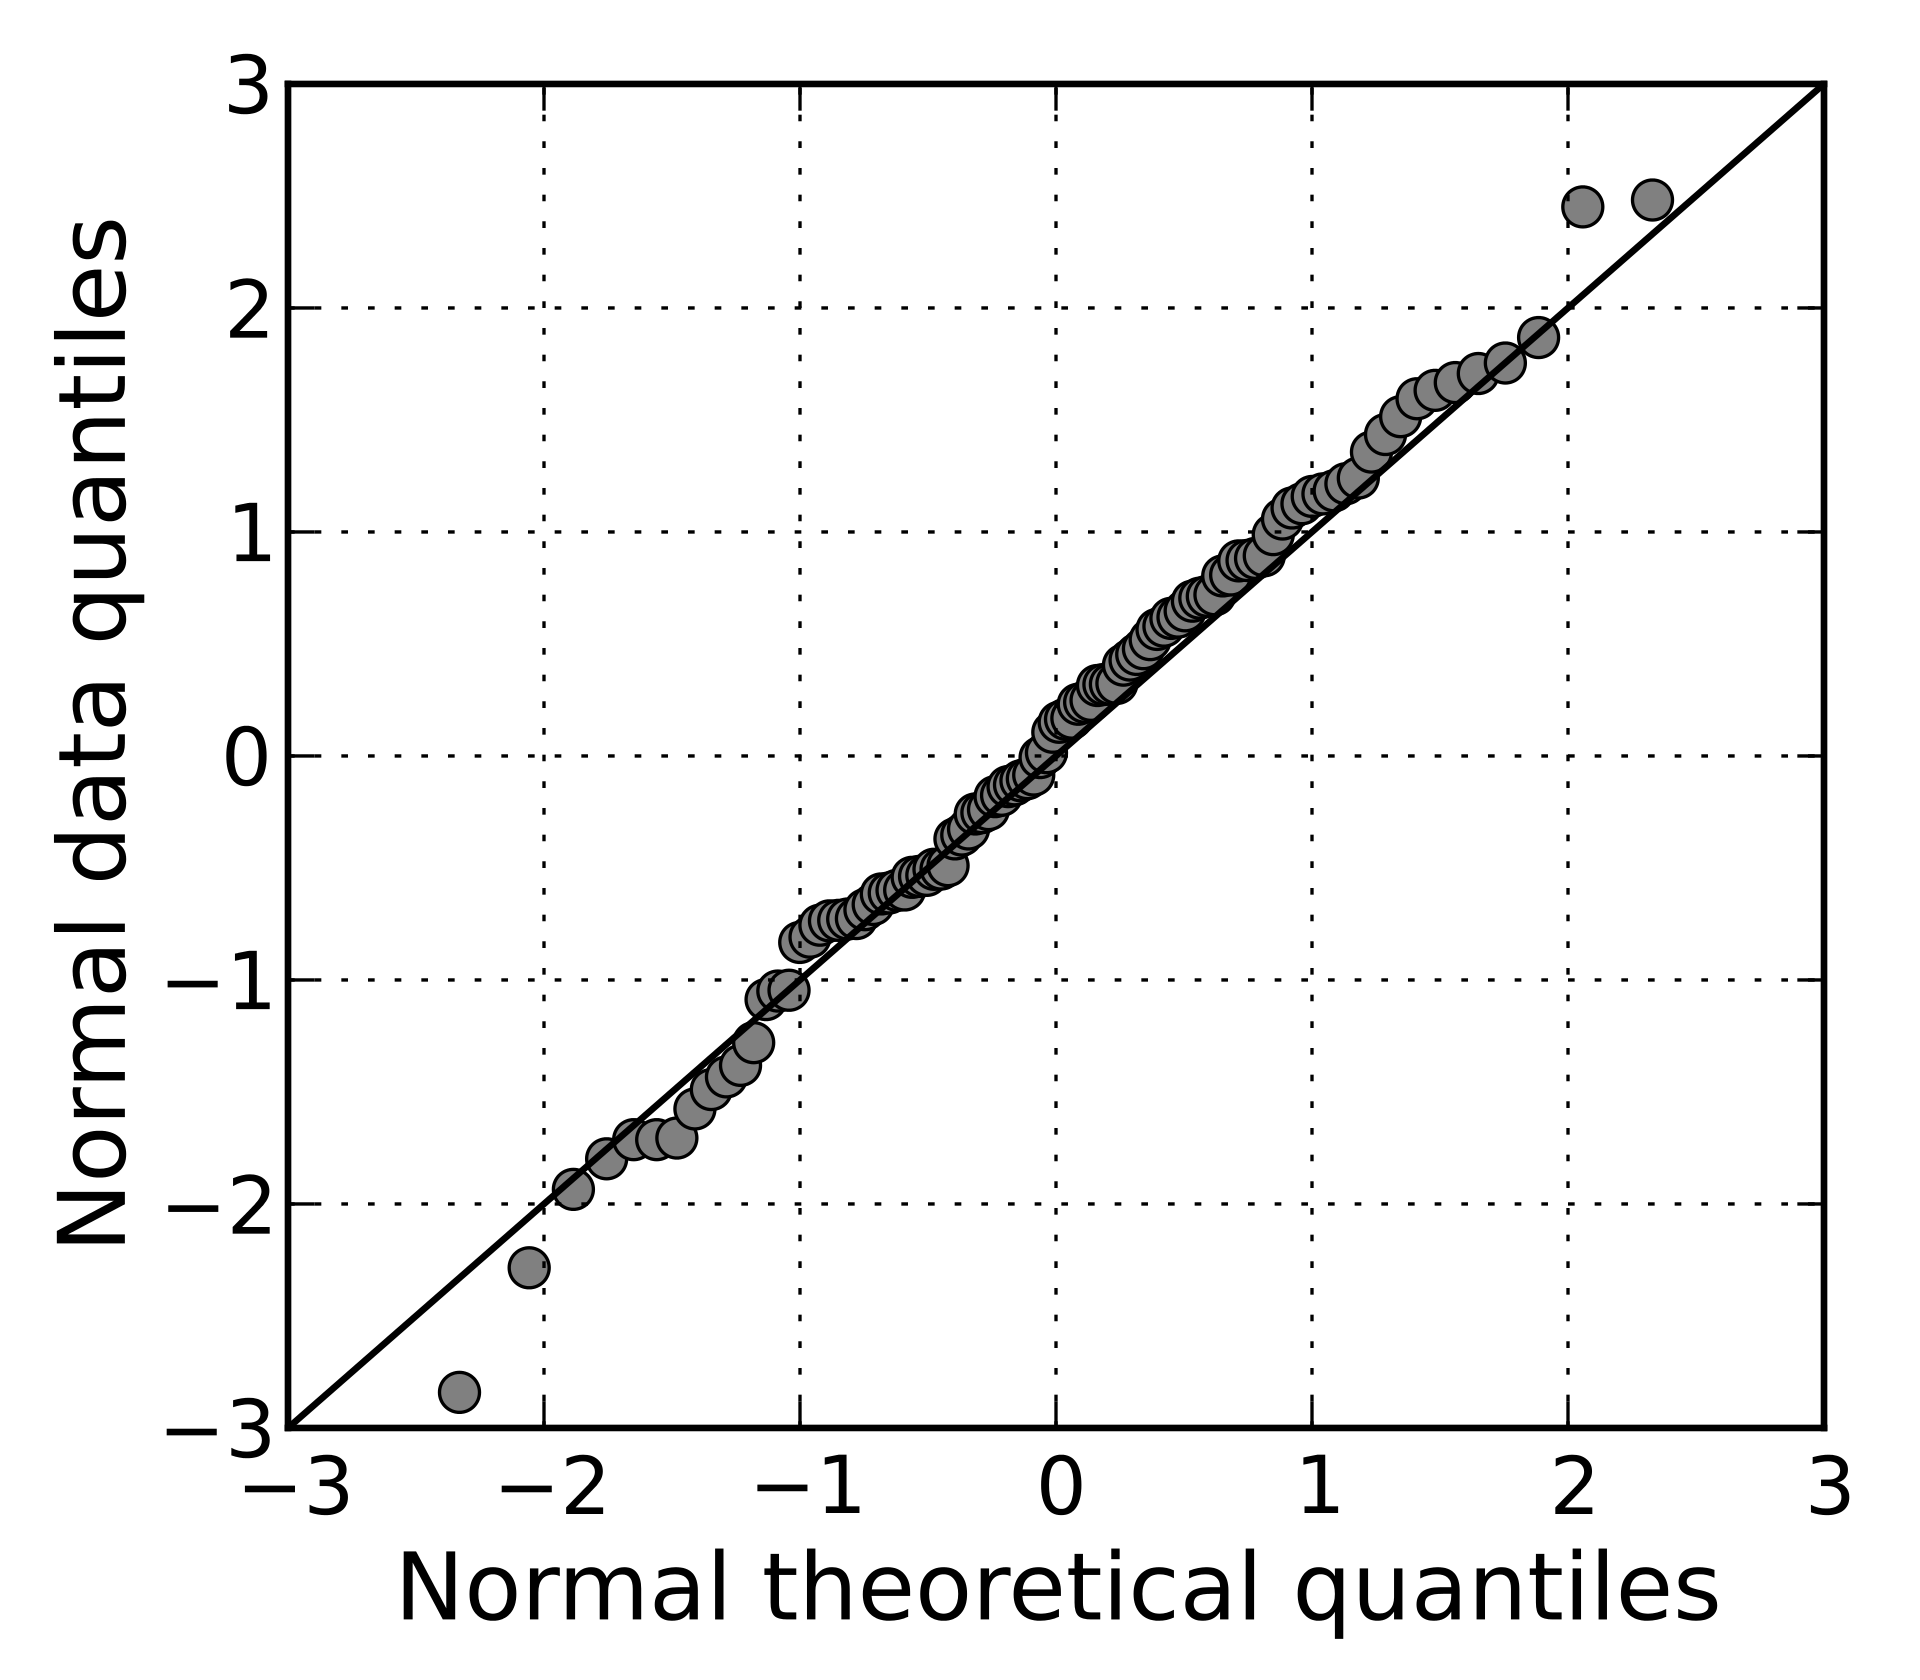
\includegraphics[width=1.5in]{normal_qq}
\end{center}

\begin{itemize}
	\item A normal probability plot using quartiles can be used to evaluate how closely a given distribution adheres to normality, where the straight line is a perfect normal curve
	\item As $N$ increases, the deviation from normality will decrease
\end{itemize}

\hformbar



\formdesc{Z Scores}

\begin{equation} Z = \frac{x - \mu}{\sigma}\end{equation}

converts any value from a normal distribution to its corresponding value on the standard normal distribution

\begin{itemize}
	\item Describes the number of standard deviations a point is from the mean $\mu$
	\item Z scores to the left of $\mu$ are negative, and positive to the right of $\mu$
\end{itemize}
\hformbar



\formdesc{Z Scores: Probabilities on Normal Distribution}

\subsection*{Ex. What is the probability $X > A$, given $X \sim N(\mu=1500, \sigma=300)$?}

\begin{equation}
	Z = \frac{x - \mu}{\sigma} = \frac{1630 - 1500}{300} = 0.43
\end{equation}

This is 0.6664 on Z table, so 66.64 percent of $X$ is to the left of A so:

\begin{equation}
	1 - 0.6664 = 0.3336
\end{equation}

The probability $X > A$ is 33.36 percent.


\subsection*{Ex. Given $A = 1400$ and $X \sim N(\mu=1500, \sigma=300)$, what is the percentile corresponding to A?}

\begin{equation}
	Z = \frac{x - \mu}{\sigma} = \frac{1400 - 1500}{300} = -0.33
\end{equation}

The corresponding value on the Z table is 0.3707, so $A$ is the 37th percentile.


\subsection*{Ex. Given $p = .40$ and $X \sim N(\mu=70, \sigma=3.3)$, what is the value corresponding to percentile $p$?}

Lookup $p$ on Z table, getting a $Z = -0.25$. Work backwards:

\begin{equation}
	-0.25 = Z = \frac{x - \mu}{\sigma} = \frac{x - 70}{3.3}
\end{equation}

and solve for $x = 69.18$.


\subsection*{Ex. What is the probability $X$ is between $A$ and $B$, given $X \sim N(\mu, \sigma)$?}

Using Z-scores method, find the area to the left of $A$ and to the right of $B$, then $A - B = 1 -$ area left of $A -$ are to right of $B$.
\hformbar



\formdesc{Bernoulli Distribution}

\begin{equation}
	P(X = x) = \left\{\begin{matrix}
					  p ~$for$~ x = 1\\ 
                      1 - p ~$for$~ x =0
                \end{matrix}\right.
\end{equation}

describes the distribution of individual trials with two possible outcomes, success or failure, described by proportion of successes $0 \leq p \leq 1$:

\begin{eqnarray}
  \hat{p}   &=& \frac{\mid successes \mid}{\mid failures \mid} \\
  \mu       &=& p \\
  \sigma^2  &=& p(1 - p)
\end{eqnarray}

\begin{itemize}
	\item The probability of success after $n$ trials is $(1 - p)^{n - 1} \times p$
\end{itemize}

\hformbar



\formdesc{Bernoulli: Geometric Distribution}

\begin{center}
    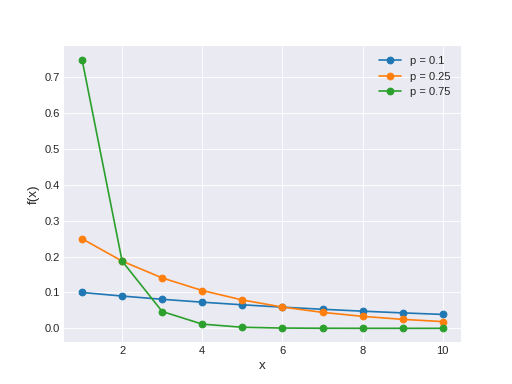
\includegraphics[width=2in]{geometric_dist}
\end{center}

describes the wait time until a success for \textit{independent} Bernoulli random variables; or, the probability of observing the $k$-th success by the $n$-th trial

\begin{eqnarray}
  \mu       &=& \frac{1}{p} \\
  \sigma^2  &=& \frac{1 - p}{p^2}
\end{eqnarray}

\begin{itemize}
	\item Higher $p$ means fewer trials until success
	\item Can never be approximated by a normal distribution
\end{itemize}

\hformbar



\formdesc{Binomial Distribution}

\begin{center}
    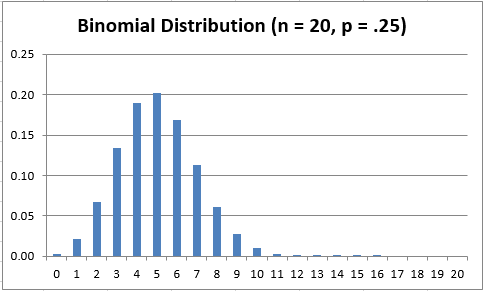
\includegraphics[width=2in]{binomial}
\end{center}

describes the probability of having exactly $k$ successes in $n$ independent Bernoulli trials (with probability of success $p$):

\begin{eqnarray}
	P(x = k \mid n, \mu, \sigma) &=& \begin{pmatrix}
		n\\ 
		k
	\end{pmatrix}
	p^k (1 - p)^{n -k} \\
	&=& \frac{n!}{k!(n - k)!} ~p^k (1 - p)^{n - k} 
\end{eqnarray}

Parameters, can be used to approximate to normal when $n$ is sufficiently large and $np$ and $n(1-p)$ are both greater than or equal to 10:

\begin{eqnarray}
  \mu       &=& np \\
  \sigma^2  &=& np(1 - p)
\end{eqnarray}

\hformbar



\formdesc{Poisson Distribution}

\begin{center}
    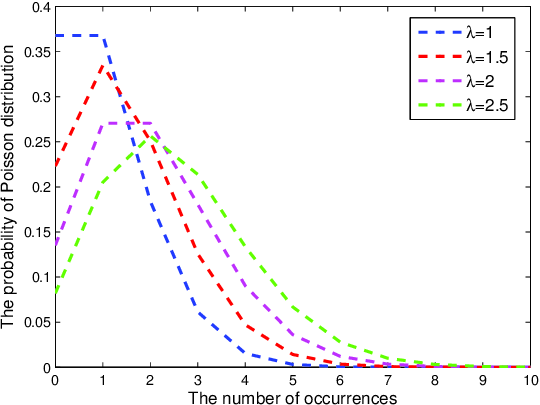
\includegraphics[width=2in]{poisson}
\end{center}

\begin{equation}
	P(X = x \mid \lambda) = \frac{\lambda^x e^{-\lambda}}{x!}
\end{equation}

Describes the number of events in a larger population over a unit of time with rate $\lambda$:

\begin{eqnarray}
  \mu       &=& \lambda \\
  \sigma^2  &=& \lambda
\end{eqnarray}

\hformbar







%%%%%%%%%%%%%%%%%%%%%%%%
%
% Inferential Statistics
%
% See Statistical Inference by Casella p. 373 for alternative and better 
% notation for this
%
%%%%%%%%%%%%%%%%%%%%%%%%























\formdesc{Inferential Statistics}

The body of thought governing the inferences of populations from samples,
and how these sample statistics can vary.
\hformbar



\formdesc{Standard Error}

\begin{equation}
	SE = \frac{\sigma}{\sqrt{n}}
\end{equation}

is the standard deviation of distributions of sample statistics, when population $\sigma$ is known. If it is unknown, and if $n > 30$, substitute sample standard deviation $s$

\begin{itemize}
	\item $SE$ decreases as $n$ increases
	\item $SE$ decreases as $\sigma$ (or $s$) decreases
\end{itemize}
\hformbar



\formdesc{Confidence Intervals}

\begin{equation}
	\bar{x} \pm z \times SE
\end{equation}

\begin{itemize}
	\item $\bar{x}$ is the sample statistic, such as sample mean
	\item $z \times SE$ is the \textit{margin of error}
	\item $z$ is the desired confidence level, e.g., $z = 1.96$ for a 95 percent confidence interval
\end{itemize}

\textit{Interpretation.} ``We are $Z$ percent confident the true population \textit{statistic} is between $A$ and $B$''; or, ``$Z$ percent of samples will have a \textit{sample statistic} between $A$ and $B$.''

\hformbar



\formdesc{Central Limit Theorem}

Given a population with a finite mean $\mu$ and a finite non-zero variance
$\sigma^2$, the sampling distribution of the mean approaches a normal
distribution with a mean of $\mu$ and a variance of $\frac{\sigma^2}{N}$, as
$N$, the sample size, increases---regardless of the shape of the parent population.
\hformbar




\formdesc{Hypothesis Testing}

\begin{table}[htp]
  \begin{center}
    \begin{tabular}{c|c}
      One-Sided      & Two-Sided       \\
      \hline
      $H_0: x = A$   & $H_0: x = A$    \\
      $H_A: x >/< A$ & $H_A: x \neq A$
    \end{tabular}
  \end{center}
\end{table}

\vspace{-2em}

The process of comparing two point estimates, to determine if any difference between them is ``real'' or the result of natural variance in samples.

\begin{itemize}
	\item \textit{Type I} errors, or false positives, occur when $H_0$  is true, but rejected
	\item \textit{Type II} errors, or false negatives, occur when $H_A$ is true, and $H_0$ is not rejected
\end{itemize}

\subsection*{Quantifying Risk}

\begin{itemize}
	\item The risk of Type I errors is quantified by $\alpha$, i.e., the probability the point estimate is more than $z^*$ standard deviations away from the true population parameter
	\item The $p$-value is the probability of observing data at least as favorable to the alternative hypothesis, i.e., as ``extreme,'' as the present data set, if $H_0$ is actually true
	\item If the $p$-value is less than the chosen $\alpha$, data is sufficient to reject $H_0$
\end{itemize}
\hformbar



\formdesc{P-Value Calculations}

\subsection*{One-Sided}

%\begin{enumerate}
%	\item Look up test statistic, e.g., $\bar{x}$, on $z$-table
%	\item Determine the probability that $Z$ is more extreme than $\bar{x}$:
%	    \begin{equation}
%	    	Z = \frac{\bar{x} - \mu}{SE}}
%	    \end{equation}
%	\item Use 
%\end{enumerate}

\subsection*{Two-Sided}

\hformbar



\formdesc{Sample Proportions}

Population parameter $\pi$ is sampled:

\begin{eqnarray}
  \mu       &=& \hat{p} = \frac{\sum_n^{i=1} x_{i}}{n} \\
  SE_{\hat{p}}  &=& \sqrt{\frac{p(1-p)}{n}}
\end{eqnarray}

where $0 \leq \hat{p} \leq 1$ and $x_i = \{0, 1\}$
\hformbar



\formdesc{Sample Proportions: Confidence Intervals}

\begin{enumerate}
	\item Assess normality:
		\begin{itemize}
			\item At least 10 observations for each $\{0, 1\}$
			\item Sample is less than 10 percent of population and observations are independent
		\end{itemize}
	\item Calculate standard error $SE_{\hat{p}} = \sqrt{\frac{p(1-p)}{n}}$
	\item Determine $z^*$, e.g., 1.96
	\item Put together point estimate and margin of error:
	\begin{equation}
		\hat{p} \pm z^* \times SE_{\hat{p}}
	\end{equation}
\end{enumerate}

\hformbar



\formdesc{Sample Proportions: Hypothesis Tests}

\textbf{FIX}

\begin{eqnarray}
  H_0: \hat{p} = 0.5 \\
  H_A: \hat{p} >/\neq 0.5
\end{eqnarray}

\begin{enumerate}
	\item Evaluate normality
	\item Compute $SE_{\hat{p}}$ \textit{using null hypothesis}:
		\begin{equation}
			SE_{\hat{p}} = \sqrt{\frac{p(1-p)}{n}},
		\end{equation}
		often $ \sqrt{\frac{0.5(1-0.5)}{n}}$
	\item Calculate Z-score using hypotheses:
		\begin{equation}
			\frac{\hat{p} - \hat{p}_0}{SE_{\hat{p}}}
		\end{equation}	
	\item Convert $Z$ to $p$-value and decide whether to reject the null or fail to
\end{enumerate}

\hformbar



\formdesc{Sample Proportions: Sample Size}
\hformbar



\formdesc{Difference of Proportions}
\hformbar



\formdesc{Difference of Proportions: Confidence Intervals}
\hformbar



\formdesc{Difference of Proportions: Hypothesis Tests}
\hformbar



\formdesc{Difference of Proportions: Pooled Proportion}
\hformbar



\formdesc{$\chi^2$ goodness of fit}


\begin{equation}
	\chi^2 = \sum_{k=1}^N \frac{ (observed_k - expected_k)^2 }{ expected_k }
\end{equation}

\begin{itemize}
	\item $k$ mutually exclusive classes
	\item $n$ observations of $x_i$
	\item one parameter, degrees of freedom $df$
	\item follows the chi-square distribution if null hypothesis is true
\end{itemize}

Summarizes how strongly observed count data deviates from the expected, or null, counts---larger values of $\chi^2$ indicate stronger deviation

\subsection*{Does a statistical model fit this sample?}

\begin{enumerate}
	\item Develop hypotheses:
		\begin{enumerate}
			\item $H_0$: Sample follows distribution $D$
			\item $H_A$: Sample does not follow distribution $D$
		\end{enumerate}
	\item Check assumptions
		\begin{enumerate}
			\item Each expected count must be at least 5
			\item Can use binning to get around this
		\end{enumerate}
	\item Establish expected counts (expected proportion of total count in each bin):
		\begin{equation}
			E_k = expected_k \times n
		\end{equation}
	\item Compute $\chi^2$ statistic
	\item Validate assumptions hold to apply $\chi^2$ to $\chi^2$ distribution
	\item Using $k-1$ degrees of freedom, use $\chi^2$ table to compute a $p$-value
	\item Decide to reject or fail to reject $H_0$
\end{enumerate}

\hformbar



\formdesc{$\chi^2$: $p$-value}
\hformbar



\formdesc{Two-Way Tables: Independence}
\hformbar


















%%%%%%%%
%
% Trash?
%
%%%%%%%%


\formdesc{Sample Statistics: Mean and Variance}

\begin{itemize}
  \item $\mu_M = \mu$ is the mean of the sampling distribution of means
  \item $\sigma_M^2 = \frac{\sigma^2}{N}$ is the variance of the sampling
	distribution of the mean
  \item $\sigma_M = \frac{\sigma}{\sqrt{N}}$ is the standard error of the sampling
	distribution of the mean
\end{itemize}

As $N$ increases, variance of sample mean decreases
\hformbar




\formdesc{Sample Statistics: Difference in Mean}

Two samples from a population the size $n_1$ and $n_2$, calculate the means
$M_1$ and $M_2$, and the difference is $M_1 - M_2$

\begin{eqnarray}
  \mu_{M_1 - M_2} &=& M_1 - M_2 \\
  \sigma_{M_1 - M_2}^2 &=& \sigma_{M_1}^2 + \sigma_{M_2}^2 \\
  \sigma_{M_1 - M_2} &=& \sqrt{\frac{\sigma_1^2}{n_1} + \frac{\sigma_2^2}{n_2}}
\end{eqnarray}

When variance and sample size are the same, standard error becomes:

\begin{equation}
  \sigma_{M_1 - M_2} = \sqrt{\frac{\sigma_1^2}{n_1} + \frac{\sigma_2^2}{n_2}}i
  = \sqrt{ \frac{\sigma^2}{n} + \frac{\sigma^2}{n}}
  = \sqrt{ \frac{2 \sigma^2}{n} }
\end{equation}

If $n_1 \neq n_2$ then variance becomes:

\begin{equation}
  \sigma_{M_1 - M2}^2 = \frac{\sigma_1^2}{n_1} + \frac{\sigma_2^2}{n_2}
\end{equation}

\subsection*{What is the probability that the mean of sample 1 will exceed that of
sample 2 by $N$ or more?}

\begin{enumerate}
  \item Find mean: $\mu_{M_1 - M_2} = M_1 - M_2$
  \item Find standard error: $\sigma_{M_1 - M_2}$
  \item Find area underneath distribution of sample 1 to the right of the mean
	of sample 2 plus $N$
\end{enumerate}

\hformbar



\formdesc{Sample Statistics: $r$ and $\rho$}

\begin{itemize}
  \item Not normally distributed---right-skewed---because correlation cannot
	exceed 1
  \item As $\rho$ increases, the more right-skewed the distribution
\end{itemize}

\hformbar



\formdesc{Sample Statistics: Proportion $\pi$}

Sampling proportion is closely related to the binomial distribution---the
total number of successes---where $p$ is the distribution of the mean number of
successes

\begin{eqnarray}
  \mu_p &=& \pi \\
  \sigma_p &=& \frac{\sqrt{N \pi (1 - \pi)}}{N}
           = \sqrt{\frac{\pi (1 - \pi)}{N}}
\end{eqnarray}

\subsection*{Find probability $p$ is greater than $A$}

Given $N$ and population proportion $\pi$:

\begin{enumerate}
  \item Find mean of $p = \pi$
  \item Calculate standard error as above
  \item Conduct as normal distribution given $N$ is sufficiently large and $\pi$
	is not too close to 0 or 1
\end{enumerate}

\hformbar



\formdesc{Estimation}

The process of estimating population parameters from sample statistics. Usually
results in a point estimate as well as interval estimates called confidence
intervals.

\hformbar



\formdesc{Degrees of Freedom}



\hformbar




\newpage
